%
% teil3.tex -- Resultate und Ausblick
%
% (c) 2022 Fabian Dünki, Hochschule Rapperswil
%
\section{Resultate
\label{0f1:section:teil3}}
\rhead{Resultate}
Im Verlauf des Seminares hat sich gezeigt, 
das ein einfacher mathematischer Algorithmus zu implementieren gar nicht so einfach ist.
So haben alle drei umgesetzten Ansätze Probleme mit grossen negativen x in der Funktion $\mathstrut_0F_1(;b;x)$.
Ebenso wird, je grösser der Wert x wird $\mathstrut_0F_1(;b;x)$, desto mehr weichen die berechneten Resultate
von den Erwarteten ab. \cite{0f1:wolfram-0f1}

\subsection{Auswertung
\label{0f1:subsection:auswertung}}
\begin{figure}
    \centering
    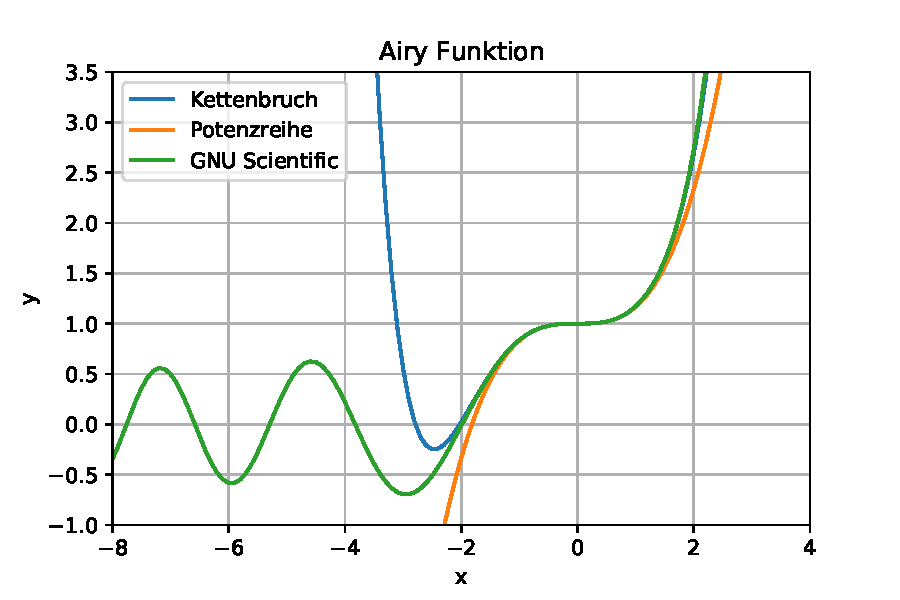
\includegraphics[width=0.8\textwidth]{papers/0f1/images/konvergenzAiry.pdf}
    \caption{Konvergenz nach drei Iterationen, dargestellt anhand der Airy Funktion zu den Anfangsbedingungen $y(0)=1$ und $y'(0)=0$.
    \label{0f1:ausblick:plot:airy:konvergenz}}
\end{figure}

\begin{figure}
    \centering
    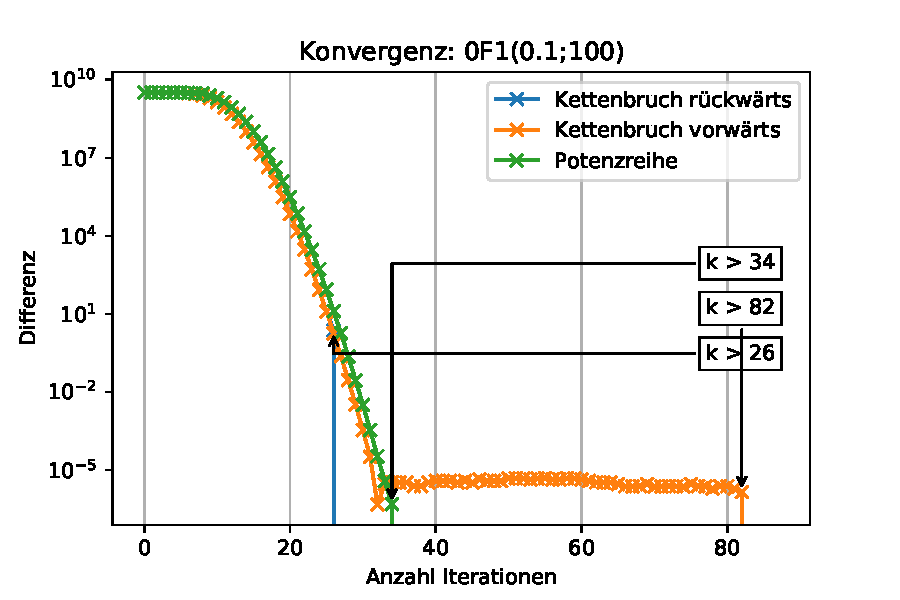
\includegraphics[width=0.8\textwidth]{papers/0f1/images/konvergenzPositiv.pdf}
    \caption{Konvergenz: Logarithmisch dargestellte Differenz vom erwarteten Endresultat.
    \label{0f1:ausblick:plot:konvergenz:positiv}}
\end{figure}

\begin{figure}
    \centering
    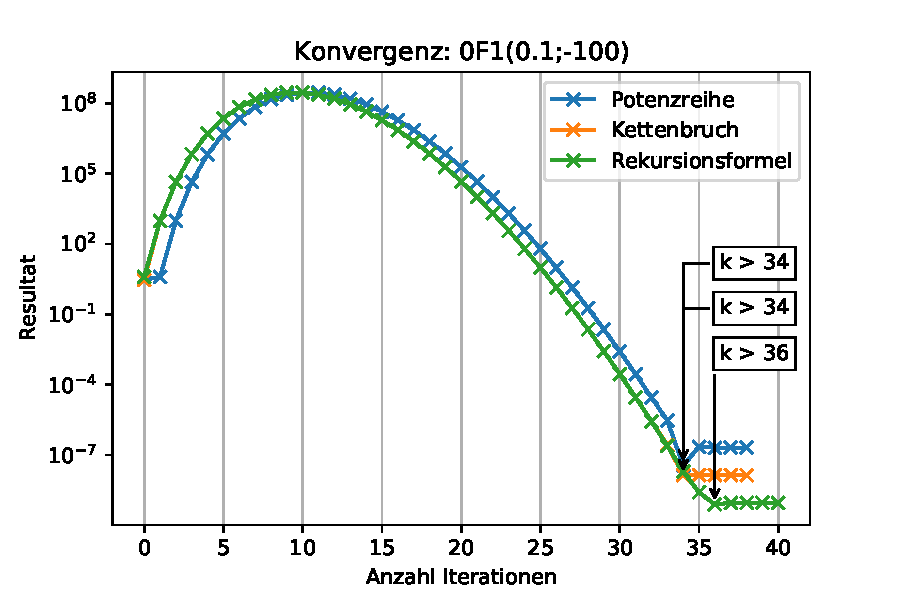
\includegraphics[width=0.8\textwidth]{papers/0f1/images/konvergenzNegativ.pdf}
    \caption{Konvergenz: Logarithmisch dargestellte Differenz vom erwarteten Endresultat.
    \label{0f1:ausblick:plot:konvergenz:negativ}}
\end{figure}

\begin{figure}
    \centering
    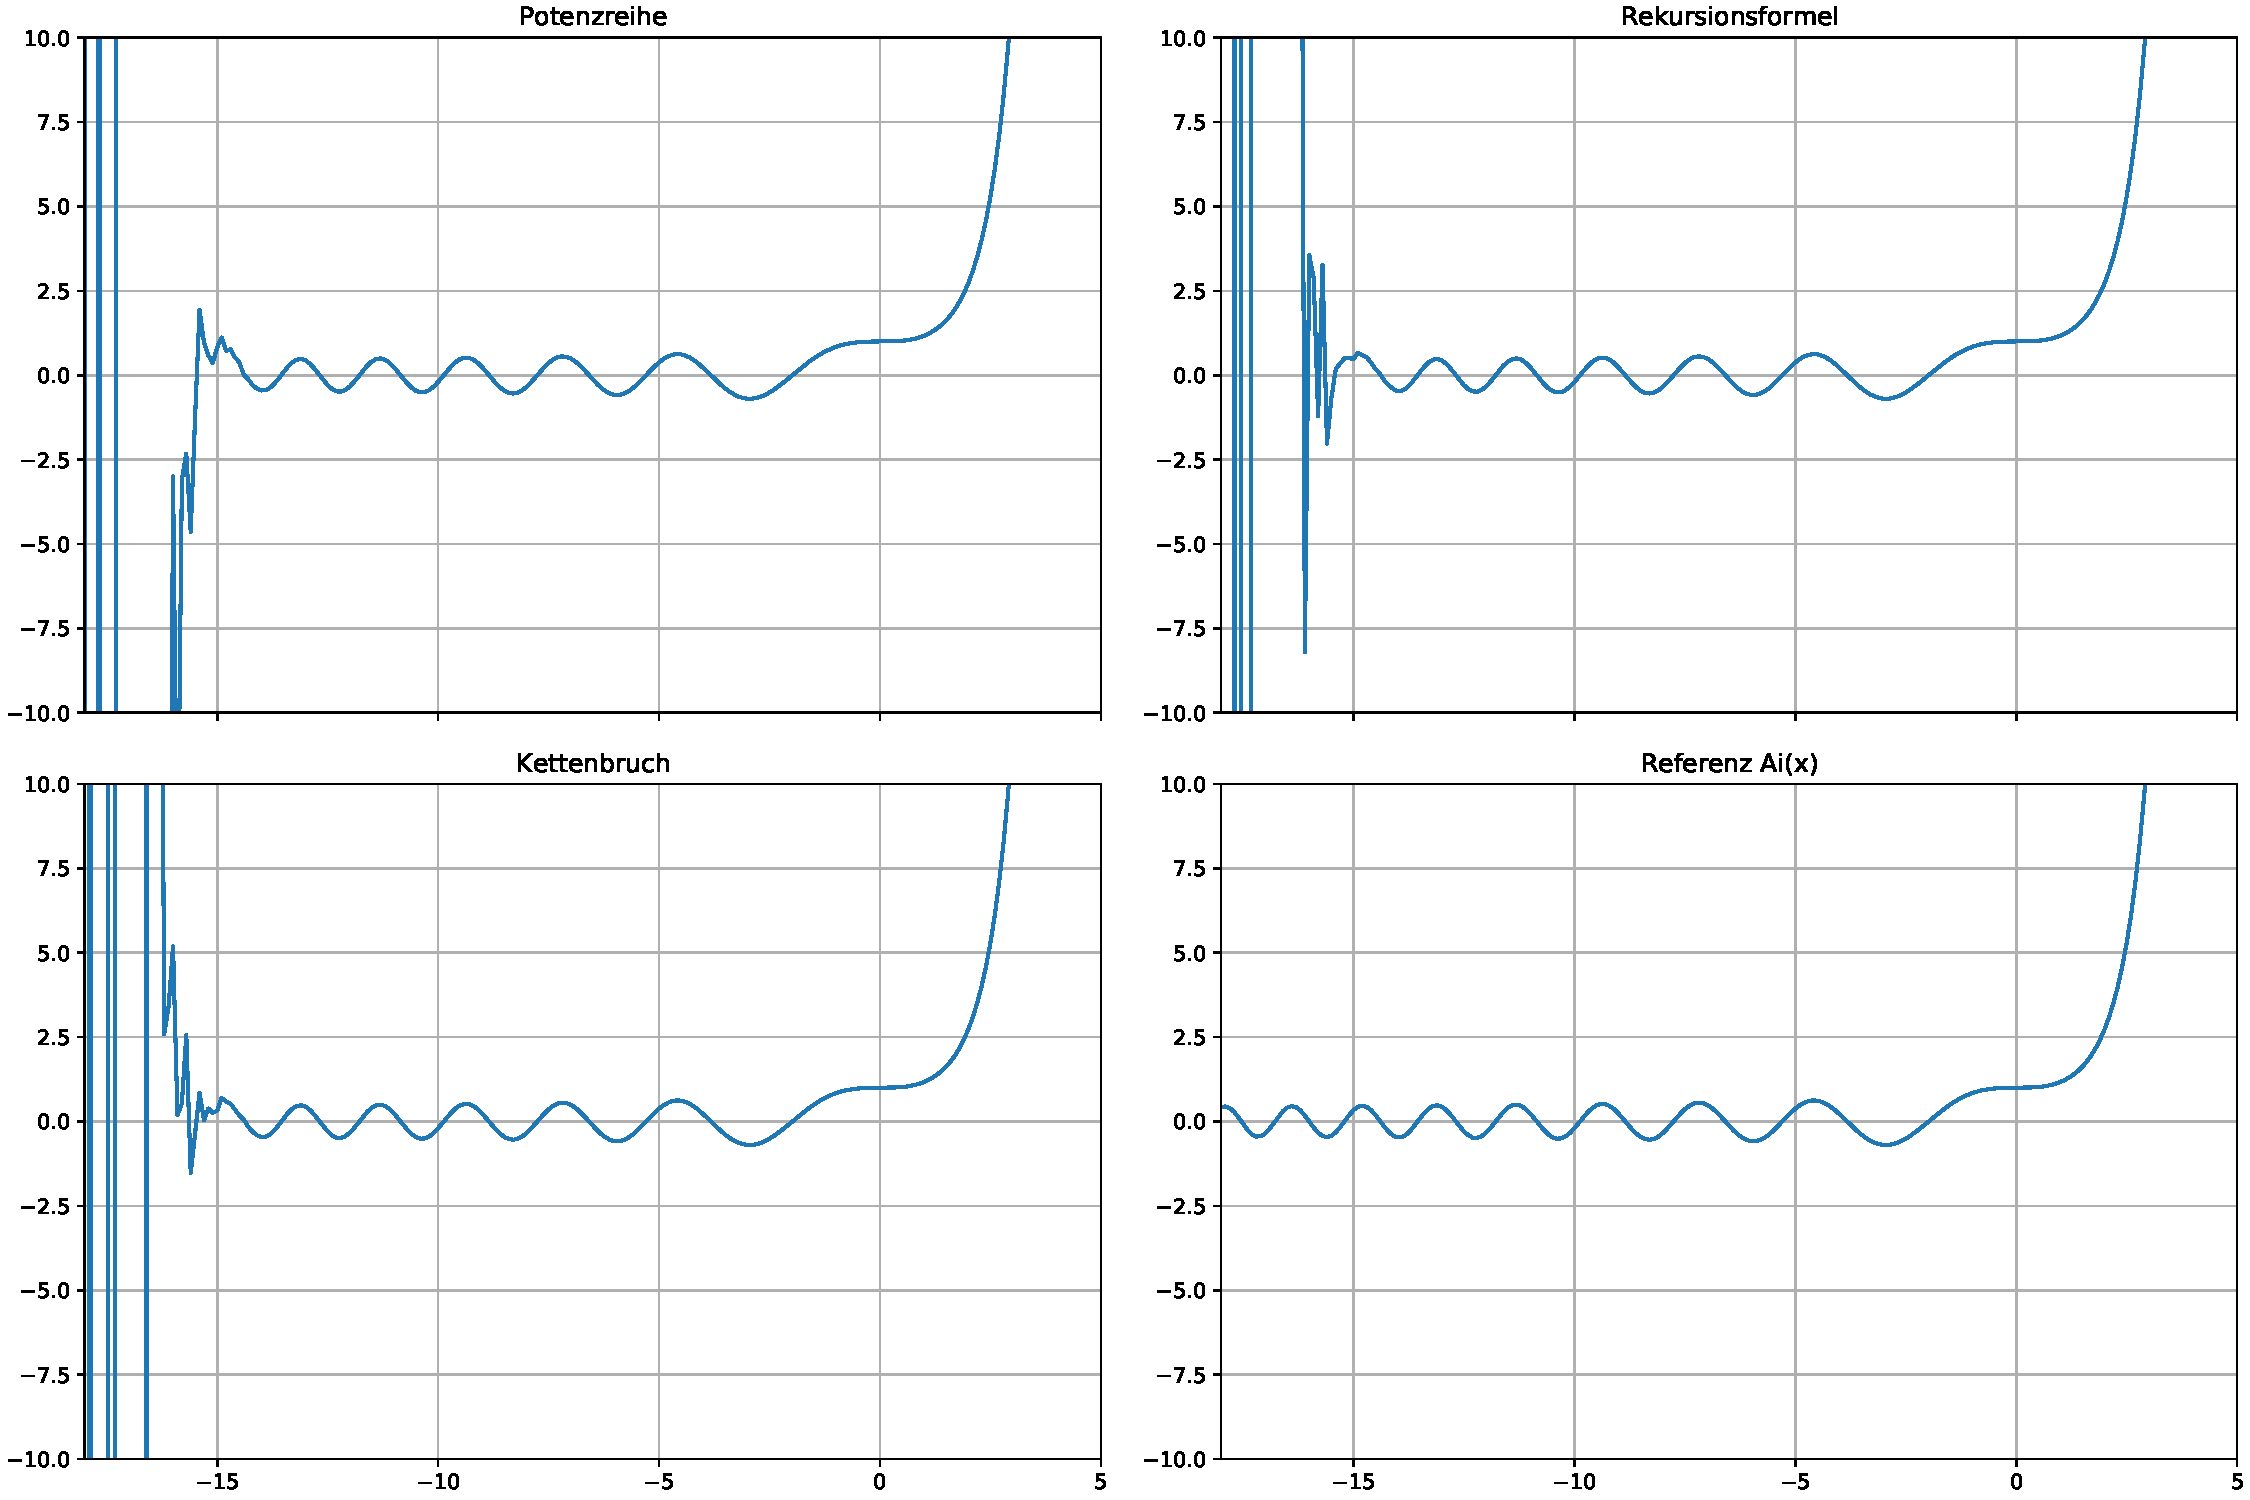
\includegraphics[width=1\textwidth]{papers/0f1/images/stabilitaet.pdf}
    \caption{Stabilität der 3 Algorithmen verglichen mit der GNU Scientific Library.
    \label{0f1:ausblick:plot:airy:stabilitaet}}
\end{figure}

\begin{itemize}
    \item Negative Zahlen sind sowohl für die Potenzreihe als auch für den Kettenbruch ein Problem.
    \item Die Potenzreihe hat das Problem, je tiefer die Rekursionstiefe, desto mehr machen die Brüche ein Problem. Also der Nenner mit der Fakultät und dem Pochhammer Symbol.
    \item Die Rekursionformel liefert für sehr grosse positive Werte die genausten Ergebnisse, verglichen mit der GNU Scientific Library.
\end{itemize}


\subsection{Ausblick
\label{0f1:subsection:ausblick}}
Eine mögliche Lösung zum Problem ist \cite{0f1:SeminarNumerik}
{\color{red} TODO beschreiben Lösung}

